% ********** Dark Results Chapter **********
\chapter{Results: Dark Measurements}
\label{cha:darkResults}
\epigraph{`The most exciting phrase to hear in science, the one that heralds new discoveries, is not `Eureka!' but `That's funny\ldots'.'}{\mbox{\textup{---\textsc{Isaac Asimov}}}}
%
\section{Introduction}\label{sec:darkresults_introduction}
The first stage of device testing was to characterise the device in the absence of any optical signal. These tests were performed in the first of the two cryogenic systems described in Chapter~\ref{cha:testbeds}. The purpose of these tests were: firstly, to ascertain that the detectors had been fabricated correctly, that is to say that a Schottky contact had formed between the aluminium and the doped silicon; the second goal of these measurements was to produce a set of data to which later---optical---data could be compared. The characterisation performed in these measurements concentrated on the current-voltage relationship of the detectors at various different bath temperatures. Attempts were also made to measure the device noise at this point; however, it was found that the amplifier noise of the readout circuitry used at the time dominated these measurements.\footnote{This was the reason the system described in Section~\ref{sec:cross_col_noise} was devised.}
%
\section{Unstrained Silicon}\label{sec:darkControlSi}
It is logical to start the exploration of silicon cold-electron bolometers with the devices fabricated from the unstrained (but still highly-doped) silicon material; the structure of these devices has already been illustrated in Figure~\ref{fig:CEB_crossSection}. This device could be thought of as offering a benchmark to which the performance of a detector utilising strained silicon could be compared. Inspection of Equation~\ref{res:NEP_CEB} shows immediately that a key limiting parameter to the noise-equivalent power is the electron-phonon coupling, $\varSigma$; Table~\ref{tab:materialProperties} shows that this parameter is substantially larger for an unstrained detector compared to a detector using strained silicon (by a factor of 26, in fact). From this, it is immediately clear that one should expect the detector described in this section to be less sensitive than the detector utilising strained silicon, which is described later in this chapter. Furthermore, Equations~\ref{res:Iresponsivity} and \ref{res:Vresponsivity} show that the responsivity, in either bias regime, is decreased for increased electron-phonon coupling, further increasing the noise-equivalent power (reducing the detectors sensitivity).
\par 
The \glsfirst{acr:IV} characteristics of the unstrained-\gls{acr:SiCEB} have been tested in the pulse-tube-cooled system detailed in Section~\ref{ssec:Aloysius} and were performed with the bias and readout system described in Section~\ref{sec:Final_Readout}. The current-voltage characteristics at various bath temperatures are shown in Figure~\ref{fig:controlIVs}.
\begin{figure}[tb]
\begin{center}
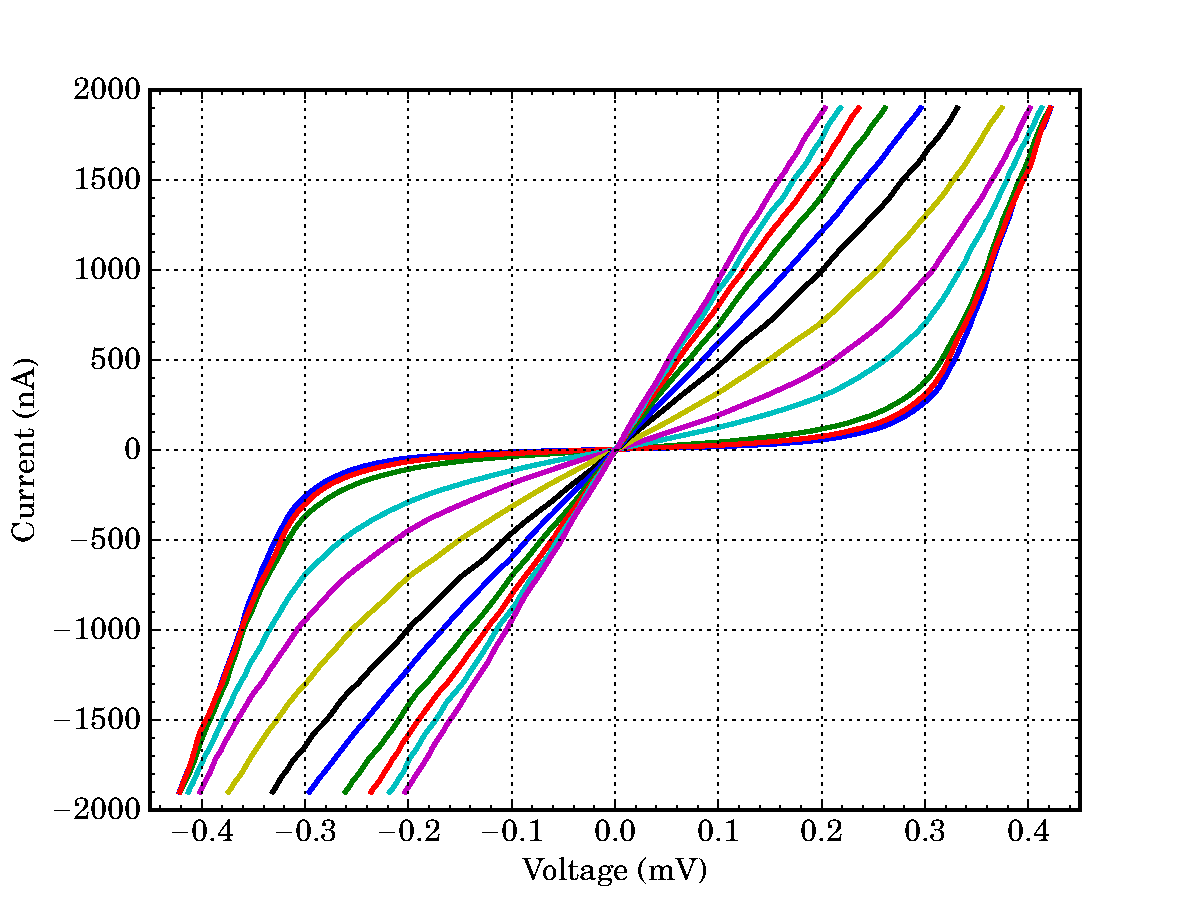
\includegraphics[width = 0.95\textwidth]{figures/control_IVs}
\caption[Current-voltage characteristics for a \gls{acr:SiCEB} with an unstrained absorber]{Current-voltage characteristics for a \gls{acr:SiCEB} with an unstrained absorber at various bath temperatures. Bath temperature from outermost (blue) to innermost (magenta, second occurrence): $0.30$, $0.35$, $0.40$, $0.45$, $0.50$, $0.60$, $0.70$, $0.80$, $0.90$, $1.00$, $1.10$, and $1.20~\mathrm{K}$.}
\label{fig:controlIVs}
\end{center}
\end{figure}
\par 
Examination of Figure~\ref{fig:controlIVs} shows that, for low bath temperatures, the \gls{acr:IV} curve is highly non-linear. The low voltage area corresponds to where the Fermi level in the silicon aligns with the energy gap within the superconductor and thus electrons cannot tunnel out of the silicon absorber into the superconducting contacts (this corresponds to the scenario shown in Figure~\ref{fig:IVmod:energyLevels-noBias}). As the voltage across the device increases, the energy levels in the semiconductor and superconducting contacts are rearranged, such that the Fermi level within the semiconductor corresponds to the vacant states above the superconducting energy gap, allowing carriers to exit the semiconductor via the tunnelling contacts (the arrangement shown in Figure~\ref{fig:IVmod:energyLevels-+Bias}). This change is seen in the \gls{acr:IV} curve by the increased gradient (lower resistance) at higher biases. At the highest biases, where the Fermi level in the semiconductor is well above the superconductor's energy gap, the \gls{acr:IV}  curve is linear, with a resistance determined by the sum of the two tunnelling resistances and the resistance of the silicon absorber itself. It should be mentioned that the data quality in Figure~\ref{fig:controlIVs} is lower than might have been desired; this has been attributed to contamination of the signals within the pulse-tube cooled testbed. Specifically, it is believed that this was caused by microphonic noise introduced by the pulse tube cooler, combined with pickup from the refrigerator control and monitoring circuitry. As will be seen later in this chapter, these issues were addressed for later, more critical, measurements.
\par 
As the bath temperature was increased (the outermost curve in Figure~\ref{fig:controlIVs} corresponds to the lowest bath temperature), it is clear that the non-linearity of the \gls{acr:IV} curve diminished. This is due to the reduction of the superconducting energy gap (as shown in Figure~\ref{fig:BCS_gap}) with increasing temperature. As the gap decreases, the energy needed to align the absorber with the vacant states above the superconducting gap decreases accordingly, until the situation where $T_{\mathrm{bath}} = T_{\mathrm{c}}$; at which point, the gap is diminished to zero and no additional energy is required for tunnelling from the absorber to the contacts. The case where $T_{\mathrm{bath}} = T_{\mathrm{c}}$ is shown by the innermost curve of Figure~\ref{fig:controlIVs}, which is entirely linear with a resistance corresponding to the tunnelling resistance (along with any contribution from the absorber and the now normal-state contacts) at all biases. 
\par 
\begin{figure}[tb]
\begin{center}
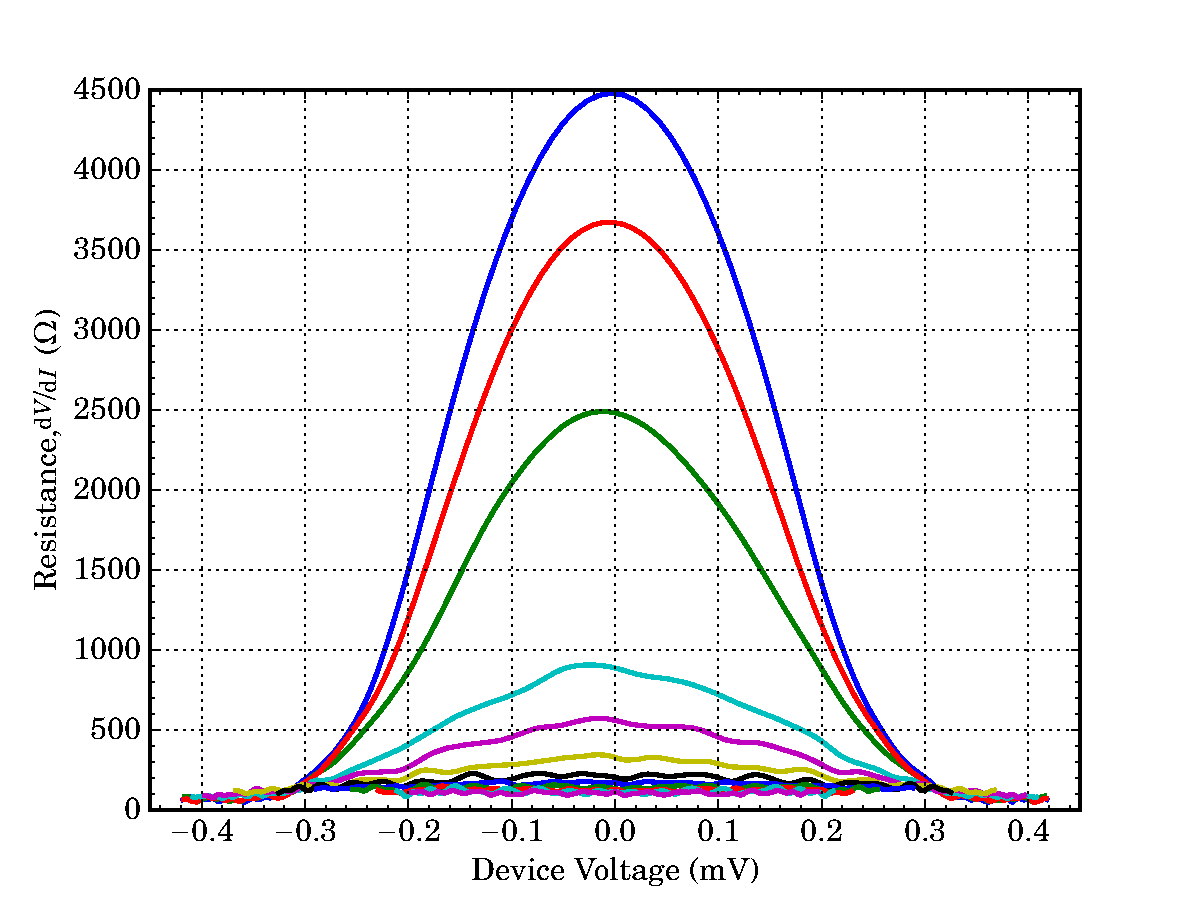
\includegraphics[width = 0.95\textwidth]{figures/control_Rderiv}
\caption[Differential resistance for a \gls{acr:SiCEB} with an unstrained absorber]{Differential resistance for a \gls{acr:SiCEB} with an unstrained absorber at various bath temperatures. Colours as in Figure~\ref{fig:controlIVs}. Bath temperature from outermost (blue) to innermost (magenta, second occurrence): $0.30$, $0.35$, $0.40$, $0.45$, $0.50$, $0.60$, $0.70$, $0.80$, $0.90$, $1.00$, $1.10$, and $1.20~\mathrm{K}$.}
\label{fig:controlRderiv}
\end{center}
\end{figure}
An alternative way of viewing the data shown in Figure~\ref{fig:controlIVs} is to calculate the differential resistance ($\nicefrac{\d V}{\d I}$) of the detector as a function of either the voltage across the detector or the current flowing through the detector. This is shown in Figure~\ref{fig:controlRderiv}.\footnote{Device voltage was selected as the x-axis of Figure~\ref{fig:controlRderiv} simply because this selection produced a clearer figure.} It is clear from this figure that, as the voltage across the detector increases, the resistance tends to the same value which is independent of the bath temperature, this value is the sum of the two tunnelling (Schottky barrier) resistances. Closer inspection of the various data found this value to be of the order $60~\mathrm{\Omega}$. This is lower than the anticipated value of $260~\mathrm{\Omega}$ which was derived from combining the anticipated contact resistance of $107~\mathrm{\Omega}$ per contact with the absorber resistance of $50~\mathrm{\Omega}$. This discrepancy was most likely due to a Schottky contact not being formed evenly throughout the contact area but instead some areas forming Ohmic contacts. From observing these data, and those presented in Figure~\ref{fig:controlIVs}, it becomes apparent that the superconducting gap was not, in fact, described by a transition temperature of for the aluminium of $T_{\mathrm{c}} = 1.20~\mathrm{K}$ as anticipated but instead a value of $T_{\mathrm{c}} = 1.05~\mathrm{K}$ describes the data better. This was most likely due to contamination of the aluminium during deposition or during storage of the device. This may also be the cause of the lower-than-expected normal-state resistance.
\par 
Using the data presented in Figure~\ref{fig:controlIVs}, it was possible to compute the electron temperature, $T_{\mathrm{e}}$ as a function of either the voltage across or current through the detector.\footnote{As previously mentioned for Figure~\ref{fig:controlRderiv}, figures have most commonly been plotted as a function of the device voltage for clarity, along with providing a clearer link to the underlying physical processes.} This has been performed by fitting the data using Equation~\ref{res:IV} with $T_{\mathrm{e}}$ as the only free parameter. In order to do this, the data first needed to be prepared by noting a few facts about Equation~\ref{res:IV} (previously discussed in Chapter~\ref{cha:theory}). Firstly, Equation~\ref{res:IV} only computes the current due to electron tunnelling through the barrier, it does not allow for the current drawn due to the series resistance of the detector's absorber, $R_{\mathrm{abs}}$; to address this, it was necessary to scale the voltage such that the current due to this resistance was removed, this voltage, $V_{\mathrm{J}}$ was simply given by:
\begin{align}
V_{\mathrm{J}} &= V_{\mathrm{CEB}} - IR_{\mathrm{abs}}\,,
\end{align} 
where $V_{\mathrm{J}}$ is the voltage dropped through the two junctions, $V_{\mathrm{CEB}}$ is the total voltage across the detector, $I$ is the current flowing through the detector, and $R_{\mathrm{abs}}$ is the resistance of the absorber. Secondly, $R_{\mathrm{N}}$ in Equation~\ref{res:IV} is the normal-state resistance of the structure (excluding the absorber resistance, as discussed above); that is to say, the resistance of tunnelling through both junctions of the detector as seen at higher biases in Figure~\ref{fig:controlIVs}. Equation~\ref{res:IV} however, computes the current due to a single junction and, as such, it was necessary to simply divide the normal-state resistance by a factor of two.\footnote{Note that Equation~\ref{res:IV} already divides the voltage by a factor of two to allow for the series arrangement of two identical junctions.}
\par 
This electron-temperature fitting has been performed for the data presented in Figure~\ref{fig:controlIVs} (using the parameters give in Table~\ref{tab:ControlTeParams_dark}) and is shown in Figure~\ref{fig:controlTe} for the three lowest bath temperatures available $0.30$, $0.35$, and $0.40~\mathrm{K}$. It is clear from this figure that the electron temperature is equal to the bath temperature at zero bias and falls to a minimum at a voltage slightly below $\nicefrac{2\varDelta}{e}$ ($\approx 0.30~\mathrm{mV}$ for this device). At voltages beyond $\approx \nicefrac{2\varDelta}{e}$, the temperature of the electrons starts to climb rapidly; this climb corresponds to the situation where a great number of carriers in the absorber have energies corresponding to the vacant states above the superconductor's energy gap and tunnelling becomes decreasing less thermally selective.
\begin{figure}[tb]
\begin{center}
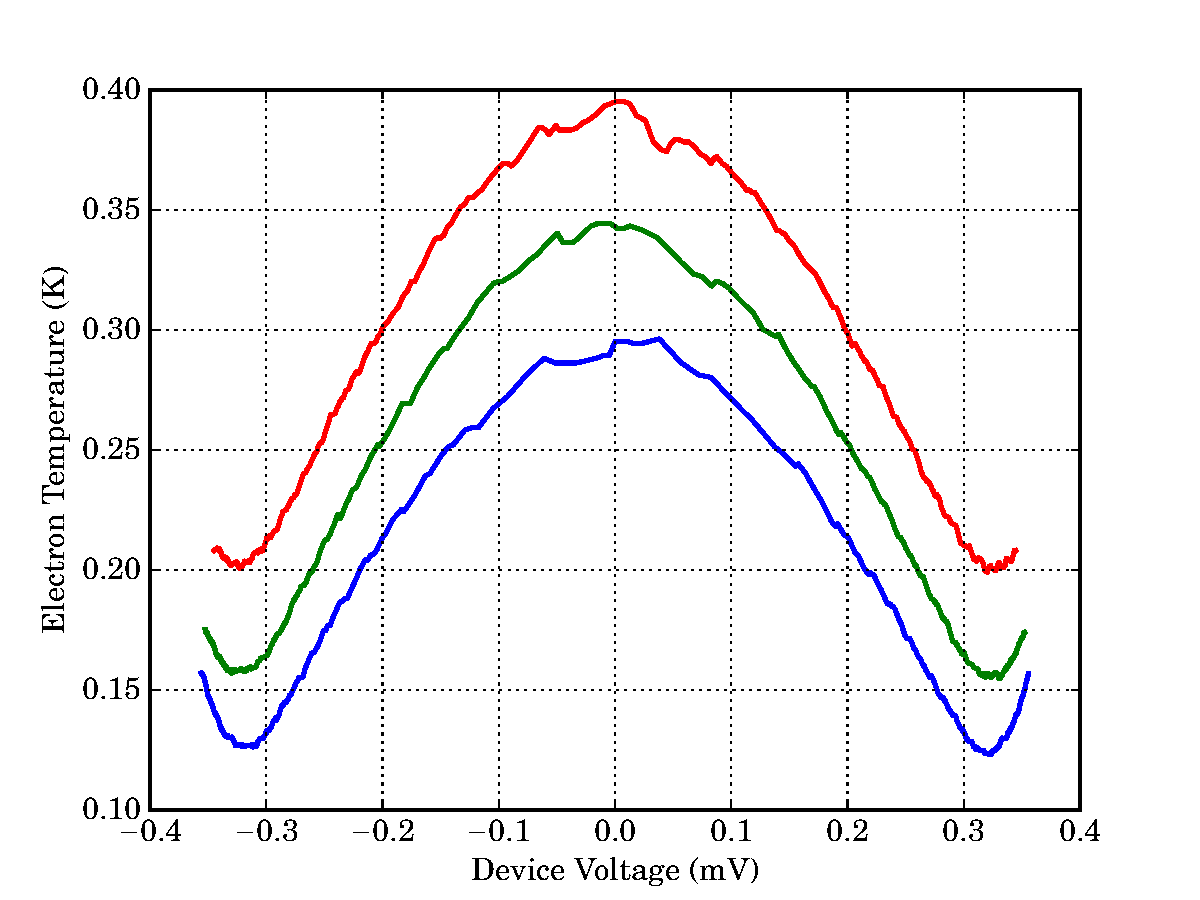
\includegraphics[width = 0.95\textwidth]{figures/control_Te}
\caption[Electron-temperature fitting for \gls{acr:SiCEB} with an unstrained absorber]{Electron-temperature fitting for \gls{acr:SiCEB} with an unstrained absorber at low bath temperatures. Bath temperatures from bottom to top: $0.30$, $0.35$, and $0.40~\mathrm{K}$. Note that $T_{\mathrm{e}} = T_{\mathrm{bath}}$ at $V = 0$.}
\label{fig:controlTe}
\end{center}
\end{figure}
\begin{table}[htb]
\caption[Parameters used in electron-temperature fitting of unstrained-silicon detector with optical loading]{Parameters used in electron-temperature fitting of unstrained-silicon detector without optical loading.} 
\label{tab:ControlTeParams_dark}
\centering
\begin{tabular}{cccccc}
\toprule\toprule
$R_{\mathrm{abs}}$ & $2R_{\mathrm{N}}$ & $V_{\mathrm{J}}$ & $\varDelta$ & $\varDelta_{T=0}$ & $T_{\mathrm{c}}$ \\ \midrule
$37~\mathrm{\Omega}$ & $60~\mathrm{\Omega}$ & $V_{\mathrm{dev}} - IR_{\mathrm{abs}}$ 
& BCS, $\varDelta\left(T_{\mathrm{e}},T_{\mathrm{c}}\right)$ & $160~\mathrm{\upmu eV}$ & $1.05~\mathrm{K}$ \\
\bottomrule
\end{tabular}
\end{table}
%
\section{Strained Silicon}
The same measurements detailed in the previous section have been performed for a detector utilising a strained-silicon absorber. The expectation for this device was that it should show an ability to access lower electron temperatures, due to reduced power flow between the phonons and the electrons in this material.
\par
The current-voltage characteristics for the strained-silicon devices are shown in Figure~\ref{fig:strainedIVs}. An immediate comparison which can be made is that the \gls{acr:IV} curves measured at the lowest temperatures are much more tightly grouped than was seen in Figure~\ref{fig:controlIVs} for the unstrained device. To illustrate this point, the inset plot in Figure~\ref{fig:strainedIVs} shows the current-voltage relationship around the area $V = \nicefrac{2\varDelta}{e}$, allowing the two coldest measurements ($T_{\mathrm{bath}} = 0.30$ and $0.35~\mathrm{K}$, the outermost blue and green curves) to be seen distinctly. Closer comparison of the unstrained and strained measurements also shows that the \gls{acr:IV} curves in Figure~\ref{fig:strainedIVs} are flatter in the sub-gap region ($V = -0.3\mbox{--}+0.3~\mathrm{mV}$); this indicates that a higher quality Schottky junction has been formed and, as a result, the so-called sub-gap leakage is reduced.
\begin{figure}[tb]
\begin{center}
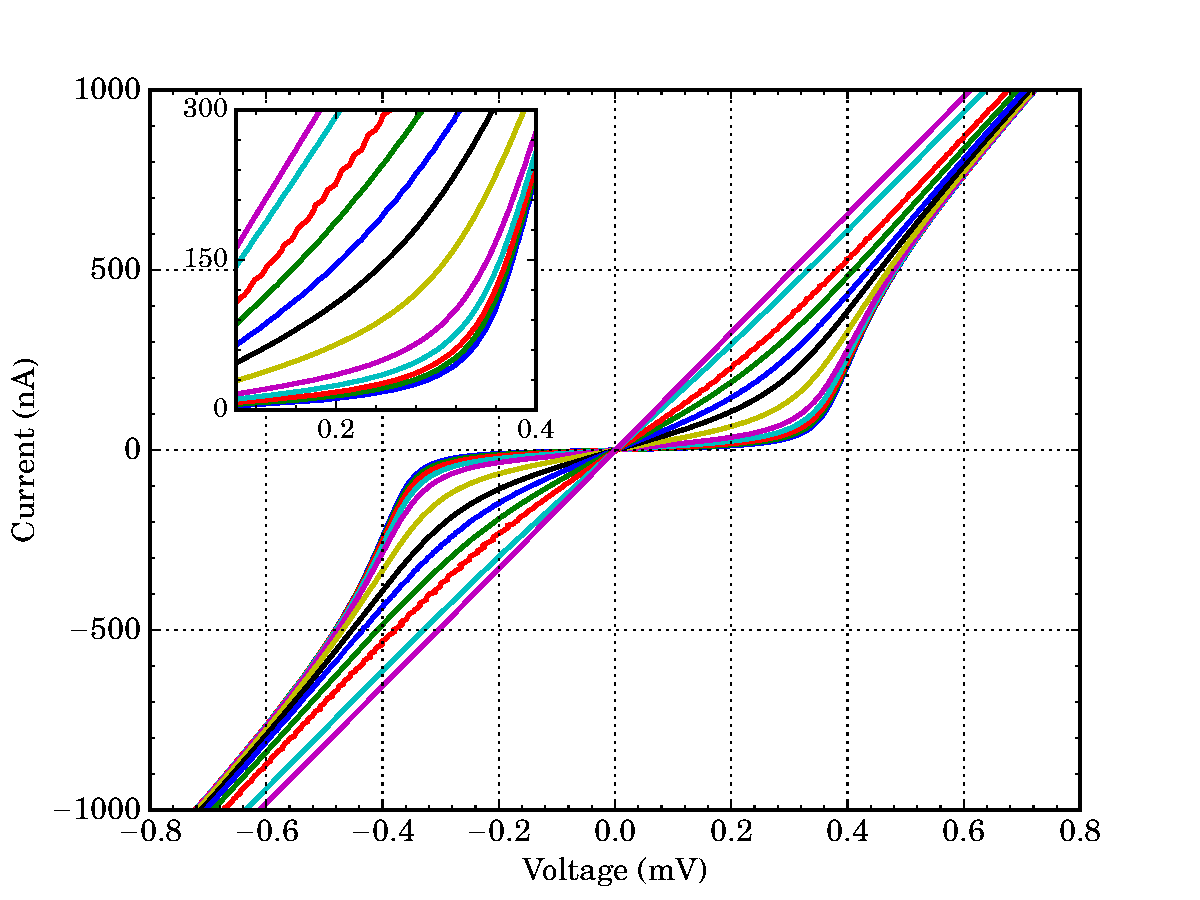
\includegraphics[width = 0.95\textwidth]{figures/strained_IVs}
\caption[Current-voltage characteristics for a \gls{acr:SiCEB} with a strained absorber]{Current-voltage characteristics for a \gls{acr:SiCEB} with a strained absorber at various bath temperatures. Inset---zoomed-in plot around voltages corresponding to $\nicefrac{2\varDelta}{e}$ to show the difference in the \gls{acr:IV} curves at the lowest bath temperatures; the axes are the same as in the main figure. Bath temperature from outermost (blue) to innermost (magenta, second occurrence): $0.30$, $0.35$, $0.40$, $0.45$, $0.50$, $0.60$, $0.70$, $0.80$, $0.90$, $1.00$, $1.10$, and $1.20~\mathrm{K}$, inset colours and areas as in main figure.}
\label{fig:strainedIVs}
\end{center}
\end{figure}
\par 
\begin{figure}[tb]
\begin{center}
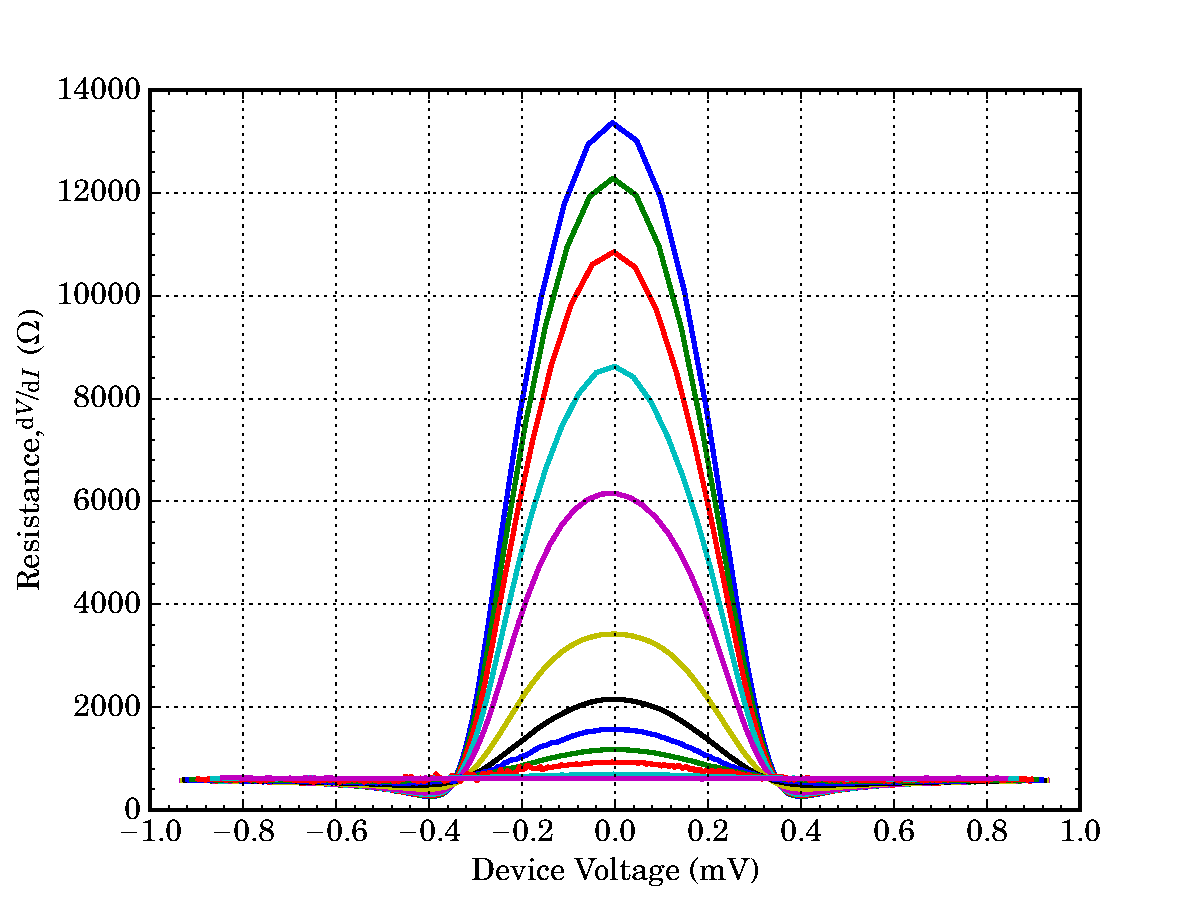
\includegraphics[width = 0.95\textwidth]{figures/strained_Rderiv}
\caption[Differential resistance of a \gls{acr:SiCEB} with a strained absorber]{Differential resistance of a \gls{acr:SiCEB} with a strained absorber at various bath temperatures. Bath temperature from top (blue) to bottom (magenta, second occurrence): $0.30$, $0.35$, $0.40$, $0.45$, $0.50$, $0.60$, $0.70$, $0.80$, $0.90$, $1.00$, $1.10$, and $1.20~\mathrm{K}$.}
\label{fig:strainedRderiv}
\end{center}
\end{figure}
Some of the key differences between these data and the previously covered data for the unstrained silicon can be seen by examining the resistance of the detector as a function of the voltage across the device (as was done in Figure~\ref{fig:controlRderiv} for the unstrained-silicon device), this is shown in Figure~\ref{fig:strainedRderiv}. Firstly, the data presented in this section indicate a critical temperature of $T_{\mathrm{c}} = 1.2~\mathrm{mK}$ for the aluminium, as was expected, and as such present an improvement over the results contained in the preceding section. The normal-state resistance of the strained-silicon device was noticeably higher than that of the unstrained detector, $580~\mathrm{\Omega}$ compared to $60~\mathrm{\Omega}$ measured for the unstrained detector. This increase was to be expected since the aluminium-silicon-junction resistance was shown in Table~\ref{tab:materialProperties} to be higher by a factor of almost $40$ for this material than for the unstrained material. The discrepancy between this value and the measured ratio of the two normal-state resistances is further indication that high-quality Schottky contacts may not have formed evenly across the entire contact area during fabrication. A further increase in the normal-state resistance was to be expected, due to the slightly higher sheet resistance of the strained material; this resulted in the absorber resistance being $75~\mathrm{\Omega}$ (compared to $50~\mathrm{\Omega}$ for the unstrained detector). This difference, however, is clearly negligible compared to the change in the contact resistance.
\par
\begin{figure}[tb]
\begin{center}
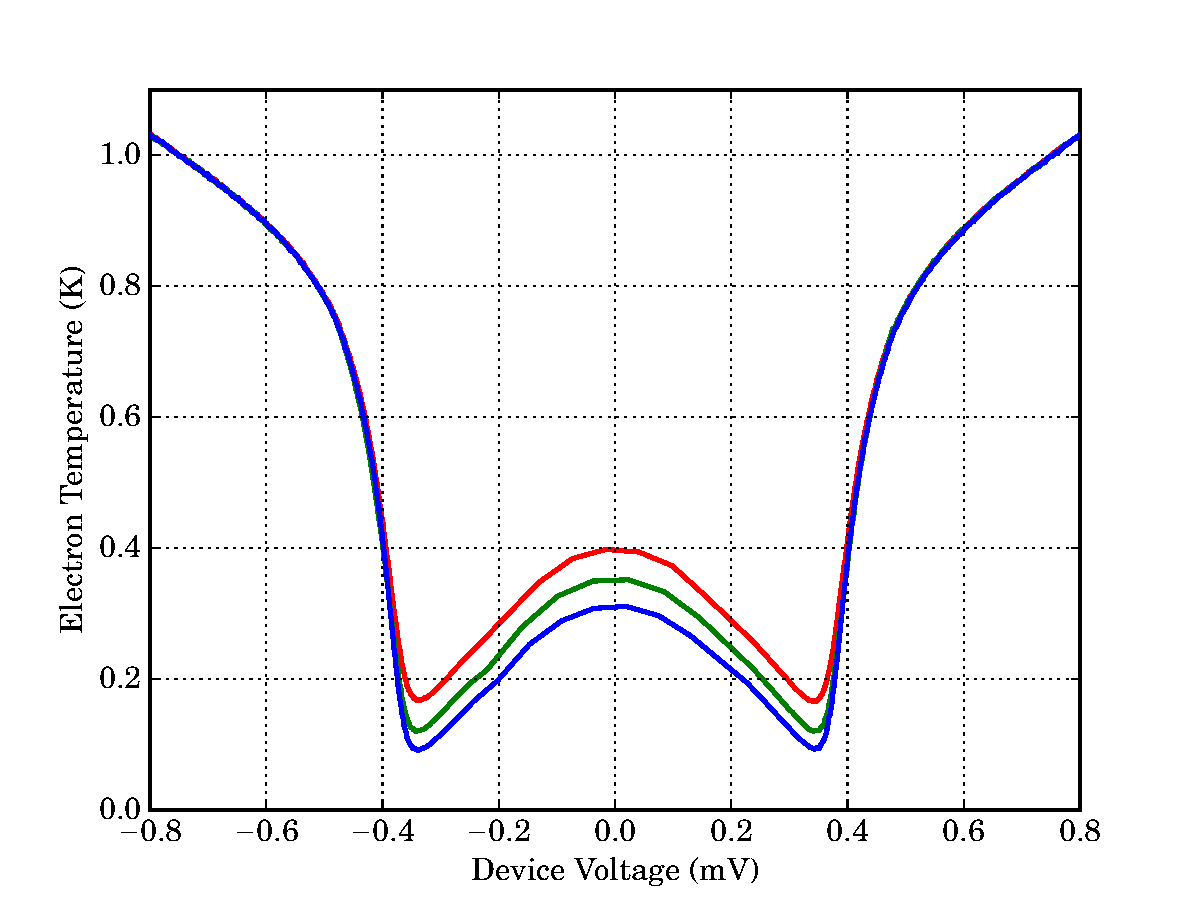
\includegraphics[width = 0.95\textwidth]{figures/strained_Te}
\caption[Electron temperature for a strained-silicon cold-electron bolometer]{Electron temperature for a strained-silicon cold-electron bolometer at low bath temperatures. Bath temperatures from bottom to top: $0.30$, $0.35$, and $0.40~\mathrm{K}$. Note that $T_{\mathrm{e}} = T_{\mathrm{bath}}$ at $V = 0$.}
\label{fig:strainedTe}
\end{center}
\end{figure}
As was performed for the unstrained-silicon device, the electron temperature has been calculated (after the previously discussed relevant changes were made) for this device. The results of this are shown for the three lowest bath temperatures ($0.30$, $0.35$, and $0.40~\mathrm{K}$) in Figure~\ref{fig:strainedTe} (the parameters used in this temperature fitting are given in Table~\ref{tab:strainedTeParams_dark}). This figure shows that at optimum bias, the device was able to self-cool to electron temperatures of $\approx 100~\mathrm{mK}$ from an initial bath temperature of $300~\mathrm{mK}$. The overall behaviour of this device seems much as expected, with the electron temperature at zero bias being set by the temperature of the phonons (the bath temperature); the minimum value of electron temperature again occurs at the situation where the absorber's Fermi level is aligned with the top of the superconducting energy gap.
\begin{table}[htb]
\caption[Parameters used in electron-temperature fitting of strained-silicon detector with optical loading]{Parameters used in electron-temperature fitting of strained-silicon detector.} 
\label{tab:strainedTeParams_dark}
\centering
\begin{tabular}{cccccc}
\toprule\toprule
$R_{\mathrm{abs}}$ & $2R_{\mathrm{N}}$ & $V_{\mathrm{J}}$ & $\varDelta$ & $\varDelta_{T=0}$ & $T_{\mathrm{c}}$ \\ \midrule
$75~\mathrm{\Omega}$ & $580~\mathrm{\Omega}$ & $V_{\mathrm{dev}} - IR_{\mathrm{abs}}$ 
& BCS, $\varDelta\left(T_{\mathrm{e}},T_{\mathrm{c}}\right)$ & $182~\mathrm{\upmu eV}$ & $1.2~\mathrm{K}$ \\
\bottomrule
\end{tabular}
\end{table}
%
\section{Comparison of Unstrained \& Strained Detectors}
\label{sec:darkComparison}
\begin{figure}[tb]
\begin{center}
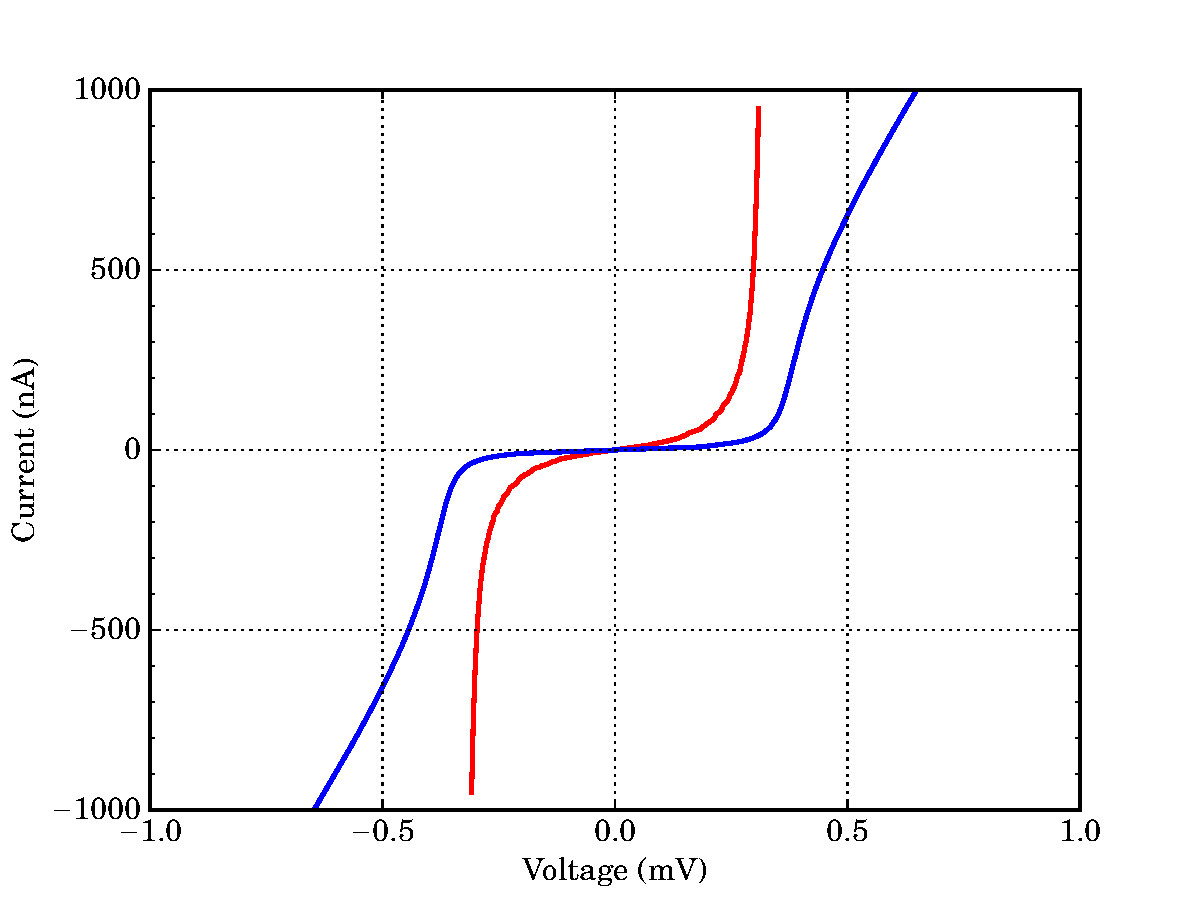
\includegraphics[width = 0.95\textwidth]{figures/IV_comparison}
\caption[Comparison of \gls{acr:IV} curves for the unstrained and strained devices]{Comparison of \gls{acr:IV} curves for the unstrained (red) and strained (blue) devices. Using \gls{acr:IV} curves measured at $300~\mathrm{mK}$}
\label{fig:IVcomparison}
\end{center}
\end{figure}
A simple comparison between the two devices tested here can be made by comparing the measured characteristics on a like-for-like basis. Comparing the current-voltage curves of the two detectors (Figures~\ref{fig:controlIVs} and \ref{fig:strainedIVs}) (as has been done, for 300-mK \gls{acr:IV} curves in Figure~\ref{fig:IVcomparison}) it can be seen that the curves for the strained-silicon detector have a much greater resistance below the superconducting gap (this point is made much more clearly from Figures~\ref{fig:controlRderiv} and \ref{fig:strainedRderiv}, which show the resistance of the device). It can also be seen that tunnelling occurs at slightly lower voltages in the unstrained device compared to the strained detector, this is not a property of the absorber but possibly a sign of a small issue with the aluminium contacts to the detector; this may also explain the lower sub-gap resistance in this device. The lower currents achieved for the strained sample are a result of the higher device resistance. As discussed earlier in this chapter, the two devices  exhibit different superconducting gap characteristics, the gap of the unstrained sample was narrower than that of the strained; this is shown clearly in Figure~\ref{fig:IVcomparison}. Since both devices used aluminium as their superconductor, this should not be the case and is attributed to contamination of the aluminium in the control detector. The difference in superconducting gap has been accounted for in all calculations in this work and the values used for the two detectors are shown in Figure~\ref{fig:materialDelta}.
\begin{figure}[tb]
\begin{center}
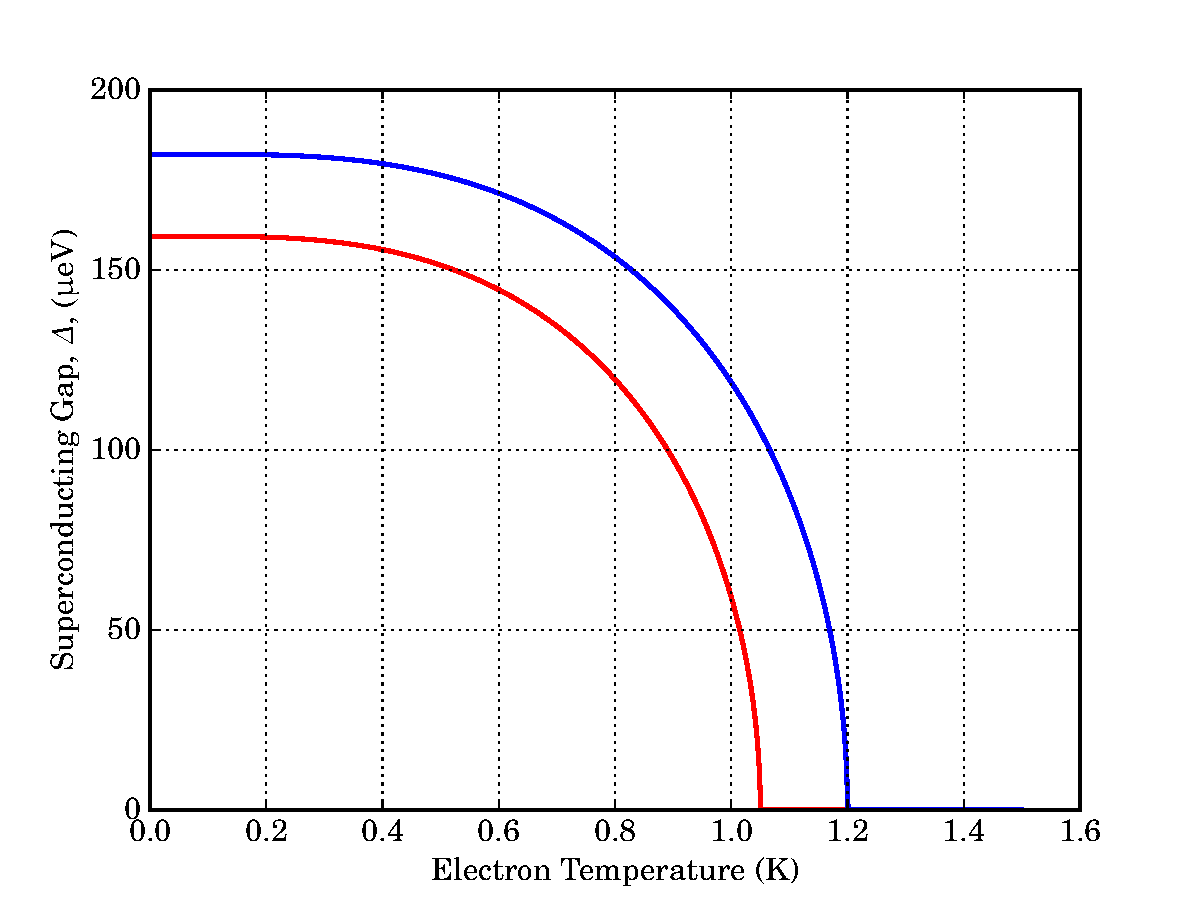
\includegraphics[width = 0.95\textwidth]{figures/SiCEB_deltaT}
\caption[Superconducting gap size as a function of temperature for the unstrained and strained devices]{Superconducting gap size as a function of temperature for the unstrained (red) and strained (blue) devices. Both devices used aluminium superconductors but the aluminium used in the unstrained device was believed to be contaminated, reducing its gap size.}
\label{fig:materialDelta}
\end{center}
\end{figure}
\par 
Comparing the electron-cooling performance of the two detectors (Figures~\ref{fig:controlTe} and \ref{fig:strainedTe}) shows that the device utilising strained silicon offered a notable reduction in the minimum achieved electron temperature. This device was able to cool carriers to a minimum temperature of $100~\mathrm{mK}$ from a bath temperature of $300~\mathrm{mK}$, compared to a minimum temperature of $170~\mathrm{mK}$ for the unstrained device operating in the same conditions. 
\par 
The results collected in this chapter indicate that the optical testing of both devices is merited, in order to compare the two materials in terms of their performance as detectors.

%\reminder[inline]{Maybe plot curves of V vs T at various biases}
